\documentclass[twoside,12pt]{article}
\newcommand{\tab}{\hspace*{2em}}
\usepackage{light}
\usepackage{subfigure}
\usepackage{graphicx}
\usepackage{amsmath}
\usepackage{verbatim}

\newcommand{\lr}{l_{right}}
\renewcommand{\ll}{l_{left}}

\newcommand{\card}[1]{\left|#1\right|}

\newcommand{\hint}[1]{({\it Hint: #1})}
\newcommand{\card}[1]{\left|#1\right|}
\newcommand{\union}{\cup}
\newcommand{\lgunion}{\bigcup}
\newcommand{\intersect}{\cap}
\newcommand{\lgintersect}{\bigcap}
\newcommand{\cross}{\times}


%\hidesolutions
\showsolutions

\newlength{\strutheight}
\newcommand{\prob}[1]{\mathop{\textup{Pr}} \nolimits \left( #1 \right)}
\newcommand{\prsub}[2]{\mathop{\textup{Pr}_{#1}}\nolimits\left(#2\right)}
\newcommand{\prcond}[2]{%
  \ifinner \settoheight{\strutheight}{$#1 #2$}
  \else    \settoheight{\strutheight}{$\displaystyle#1 #2$} \fi %
  \mathop{\textup{Pr}}\nolimits\left(
    #1\,\left|\protect\rule{0cm}{\strutheight}\right.\,#2
  \right)}
\newcommand{\comment}[1]{}
\newcommand{\cE}{\mathcal{E}}
\renewcommand{\setminus}{-}
\renewcommand{\complement}[1]{\overline{#1}}

\providecommand{\abs}[1]{\lvert#1\rvert}
\newcommand{\variance}[1]{(\Delta{#1})^2}

\begin{document}
\problemset{10}{December 4, 2012}{Monday, December 3}

%%%%%%%% f2006 PS11 P6  [Conditional probability]
\begin{problem}{5} \emph{Finalphobia} is a rare
disease in which the victim has the delusion that he or she is being
subjected to an intense mathematical examination.
%
\begin{itemize}
\item A person selected uniformly at random has finalphobia with probability
$1/100$.
\item A person with finalphobia has shaky hands with probability $9/10$.
\item A person without finalphobia has shaky hands with probability $1/20$.
\end{itemize}
%
What is the probablility that a person selected uniformly at random
has finalphobia, given that he or she has shaky hands?

\solution{
Let $F$ be the event that the randomly-selected person has
finalphobia, and let $S$ be the event that he or she has shaky hands.
A tree diagram is worked out below:
%
\begin{center}
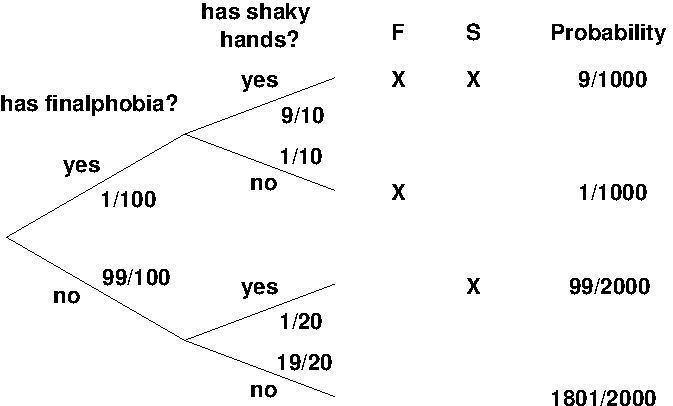
\includegraphics{finalphobia.pdf}
\end{center}
%
The probability that a person has finalphobia, given that he or she
has shaky hands is:
%
\begin{align*}
\prcond{F}{S}
    & = \frac{\pr{F \cap S}}{\pr{S}} \\
	& = \frac{\prcond{S}{F}\pr{F}}{\pr{S \cap F}+ \pr{S \cap \bar{F}}} \\
		& = \frac{\prcond{S}{F}\pr{F}}{\prcond{S}{F}\pr{F}+ \prcond{S}{\bar{F}}\pr{\bar{F}}} \\
			& = \frac{(9/10) \times (1/100)}{(9/10) \times (1/100) + (1/20) \times (99/100)} \\
	   			 & = \frac{18}{18+99} \\
	       				 & = \frac{18}{117} \text{ or } \frac{2}{13}
						\end{align*}

		So, while it's true that someone with shaky hands is five times more
		likely to have finalphobia than someone with steady hands, it remains a
		poor diagnostic for finalphobia, because only about 1 in 5 people with shaky hands actually has finalphobia.}

\end{problem}

%%%%%%%% f2010 PS11 P1 [conditional probability]
\vspace{0.15in}
\begin{problem}{9}
You are organizing a neighborhood census and instruct your census takers
to knock on doors and note the sex of any child that answers the knock.
Assume that there are two children in a household, and that girls and boys
are equally likely to be children and to open the door.

A sample space for this experiment has outcomes that are described by triples of letters: the first letter is either \texttt{B} or \texttt{G} for the sex of the elder child, likewise for the second letter denoting the sex of the younger child,
and the third letter is \texttt{E} or \texttt{Y}, indicating whether
the \emph{e}lder child or \emph{y}ounger child opened the door.  For
example, $(\mathtt{B},\mathtt{G},\mathtt{Y})$ is the outcome that the elder
child is a boy, the younger child is a girl, and the girl opened the door.

\bparts
\ppart{3} Let \emph{T} be the event that the household has two girls,
and \emph{O} be the event that a girl opened the door.  List the outcomes
in \emph{T} and \emph{O}.

\solution{$T=\set{GGE,GGY}, O=\set{GGE,GGY,GBE,BGY}$}

\ppart{3} What is the probability $\prcond{T}{O}$, that both children are
girls, given that a girl opened the door?
\solution{Two out of 4 outcomes in $O$ are also outcomes in $T$, so $\prcond{T}{O} = 1/2$.}

\ppart{3} Where is the mistake in the following argument for computing $\prcond{T}{O}$?

\begin{quote}
If a girl opens the door, then we know that there is at least one girl in
the household.  The probability that there is at least one girl is
\[
1 - \prob{\text{both children are boys}} = 1 - (1/2 \times 1/2) = 3/4.
\]
So,
\begin{eqnarray*}
\lefteqn{\prcond{T}{\text{there is at least one girl in the household}}}\\
& = & \frac{\prob{T \intersect \text{there is at least one girl in the household}}}
{\pr{\text{there is at least one girl in the household}}}\\
& = & \frac{\prob{T}}{\pr{\text{there is at least one girl in the household}}}\\
& = & (1/4) / (3/4) = 1/3.
\end{eqnarray*}
Therefore, given that a girl opened the door, the probability that there
are two girls in the household is \textup{1/3}.
\end{quote}

\solution{The argument given is a correct proof for 
\[
\prcond{T}{\text{there is at least one girl in the household}} = 1/3.
\]
The problem is that the event, $H$, that the household has at least one girl,
namely,
\[
H = \set{\mathtt{GGE,GGY,GBE,GBY,BGE,BGY}},
\]
is not the same as \emph{O}, the event that a girl opens the door.  These
two events differ:
\[
H-O = \set{\mathtt{BGE,GBY}},
\]
and consequently their probabilities are different.  So the mistake in the argument is in the final
conclusion where the value of $\prcond{T}{H}$ is taken to be the same as
the value $\prcond{T}{O}$.  Actually, $\prcond{T}{O} = 1/2$.
}

\eparts
\end{problem}


%%%%%%%% f2010 PS11 P3 /  f2008 PS11 P1 [Conditional probability]
\vspace{0.15in}
\begin{problem}{15}
With the Birthday Paradox, we found that in a group of $m$ people with $N$ possible birthdays, if $m << N$, then:
\[
\pr{\text{all $m$ birthdays are different}} \sim e^{-\frac{m(m-1)}{2N}}
\]
To find the number of people, $m$, necessary for a half chance of a matching birthday, we set the probability to $1/2$ to get:
\[
m \sim \sqrt{(2\ln2)N} \approx 1.18\sqrt{N}
\]

For $N = 365$ days we found $m$ to be 23.

We could also run a different experiment. As we write the birthday of each student surveyed on the white board, we could ask the class if anyone has the same birthday; and it's very likely that someone in the class has the same birthday as a surveyed person before we could find two surveyed students with the same birthday. Let's investigate why this would be the case.

\bparts
\ppart{5} Consider a group of $m$ people with $N$ possible birthdays amongst a larger class of $k$ people, such that $m \leq k$. Define $\pr{A}$ to be the probability that $m$ people all have different birthdays \textit{and} none of the other $k-m$ people have the same birthday as one of the $m$. Show that, if $m << N$, then $\pr{A} \sim e^{\frac{m(m-2k)}{2N}}$. Notice that the probability of no match is $e^{-\frac{m^2}{2N}}$ when $k$ is $m$, and it gets smaller as $k$ gets larger. 

\textit{Hints:} For $m << N$: $\frac{N!}{(N-m)!N^m} \sim e^{-\frac{m^2}{2N}}$, and $(1-\frac{m}{N}) \sim e^{-\frac{m}{N}}$.

\solution{
There are at least two approaches to this problem.  First, by basic counting, we find $\pr{A}$ to be
\[
\pr{A} = \frac{N(N-1)\ldots(N-m+1)\cdot(N-m)^{k-m}}{N^k}
\]

since there are $N$ choices for the first birthday, $N-1$ choices for the second birthday, etc., for the first $m$ birthdays, and $N-m$ choices for each of the remaining $k-m$ birthdays. There are total $N^k$ possible combinations of birthdays within the class.

\begin{align*}
\pr{A} &= \frac{N(N-1)\ldots(N-m+1)\cdot(N-m)^{k-m}}{N^k} \\
&= \frac{N!}{(N-m)!}\left(\frac{(N-m)^{k-m}}{N^k}\right) \\
&= \frac{N!}{(N-m)!N^m}\left(\frac{N-m}{N}\right)^{k-m} \\
&= \frac{N!}{(N-m)!N^m}\left(1-\frac{m}{N}\right)^{k-m} \\
&\sim e^{-\frac{m^2}{2N}} \cdot e^{-\frac{m}{N}(k-m)} & \text{(by the Hint)} \\
& = e^{\frac{m(m-2k)}{2N}}
\end{align*}

Another approach to this problem is to view each of $(k-m)$ people's birthdays as random variable with bernoulli distribution, where $p = \frac{m}{N}$, the probability of this birthday matching one of the $m$ people's birthdays.  Since $\pr{A} =$ Pr\{$m$ people all have different birthdays\} $\cdot$ Pr\{none of the other $k-m$ people have the same birthdays as one of the $m$\}, 
\begin{align*}
\pr{A} &\sim e^{-\frac{m^2}{2N}} \cdot (1-\frac{m}{N})^{k-m} \\
&\sim e^{-\frac{m^2}{2N}} \cdot e^{-\frac{m}{N}(k-m)} & \text{(by the Hint)} \\
&= e^{\frac{-m^2}{2N}-\frac{m(k-m)}{N}} \\
&= e^{\frac{m^2-2mk+2m^2}{2N}} \\
& = e^{\frac{m(m-2k)}{2N}}
\end{align*}
}

\ppart{5} Find $m$, the approximate number of people in the group necessary for a half chance of a match. Your answer will be in the form of a quadratic. Then simplify your answer to show that, as $k$ gets large, such that $\sqrt{N} << k$, $m \sim \frac{N\ln2}{k}$. 

\textit{Hint:} For $x << 1$: $\sqrt{1-x} \sim (1-\frac{x}{2})$.

\solution{
Setting $\pr{A} = 1/2$, we get a solution for $m$:

\begin{align*}
1/2 &= e^{\frac{m(m-2k)}{2N}} \\
-2N\ln2 &= m^2 -2km  \\
0 &= m^2-2km + (2N\ln2) \\
m &= \frac{2k \pm \sqrt{(2k)^2 - 4(2N\ln2)}}{2}
\end{align*}

Simplifying the solution under the assumption of large $k$, we find:
\begin{align*}
m &= \frac{2k - \sqrt{4k^2 - 8N\ln2}}{2} & \text{(taking the lower positive root)} \\
&= k - k\sqrt{1 - \frac{2N\ln2}{k^2}} \\
&\sim k  - k \left(1-\frac{2N\ln2}{2k^2}\right) & \text{(by the Hint)} \\
&= \frac{N\ln2}{k}  
\end{align*}
}

\ppart{5} Suppose there are 100 people in a room. Assume that their birthdays are mutually independent and uniformly distributed.
Again let $A$ be the event that two people have the same birthday. As stated in the textbook, $\prob{A} > 0.99$. Suppose we fix a particular person in the class---call her ``Jane''---and then ask everyone in the room \emph{except Jane} when their birthday is. Let $B$ be the event that all of those 99 birthdays are different.  What is the actual probability that Jane has the same birthday as another person in the room?  In other words, what is $\prcond{A}{B}$?

\solution{There are at least two ways of finding $\prcond{A}{B}$.  First, by counting, the individual outcomes in the sample space are of the form
\[
(b_1, b_2, \ldots, b_{99}, b_J)
\]
where $b_i$ is the $i$th person's birthday and $b_J$ is Jane's birthday.
The outcomes in $B$ all satisfy the property that $b_1, \dots, b_{99}$
are distinct.  Thus, by the product rule, the size of $B$ is:
\[
(365 \cdot 364 \cdots 267) \cdot 365
\]
We are interested in $\prcond{A}{B}$.
Since all outcomes have the same probability,
this is simply the fraction of outcomes in $B$ that are also in $A$.
So we're interested in the number of outcomes in $B$ satisfying $b_J \in \{b_1, \dots, b_{99} \}$.
This is
\[
(365 \cdot 364 \cdots 267) \cdot 99
\]
again by the product rule.
Thus,
\[
\prcond{A}{B}
  = \frac{(365 \cdot 364 \cdots 267) \cdot 99}{(365 \cdot 364 \cdots 267) \cdot 365}
  = \frac{99}{365} \approx 27.1\%
\]


$\begin{comment}
Old proof, using random variables:

Another way to get $\prcond{A}{B}$ treats Jane's birthday as a random variable. Let $S$ be the set of birthdays of the 99 people in the room
other than Jane. By assumption, $|S| = 99$. Let $b$ be the date
of Jane's birthday. Since $b$ is uniformly distributed over a
set of size 365, and $b$ is independent of all the birthdays in
$S$, we have
\[
\prob{A\mid B} = \prob{b\in S} = 
\frac{\card{S}}{365} = 
\frac{99}{365} \approx 27.1\%
\]

$\end{comment}
}
\eparts

\end{problem}



%%%%%%%% f2010 PS11 P5 / f2008 PS11 P3 /  f2004 PS10 + another Q from f2004 PS10  [Independence]
\vspace{0.15in}
\begin{problem}{16}   Let $A$, $B$, and $C$ be events of some experiment.

\bparts

\ppart{2} Suppose $A$ and $B$ are \emph{disjoint} events.  Prove that $A$ and
$B$ are \emph{not independent}, unless $\prob{A}$ or $\prob{B}$ is zero.

\solution{ Since $A$ and $B$ are disjoint, 
\[
\prob{A \intersect B} =  \prob{\emptyset}  = 0.
\]
So, $\prob{A \intersect B}=\prob{A} \cdot \prob{B}$ iff $\prob{A}=0$ or $\prob{B}=0$.
}


\ppart{2} If $A$ and $B$ are independent, prove that $A$ and $\bar{B}$
are also independent.  \textit{Hint:}  $\prob{A \intersect \bar{B}} = \prob{A} - \prob{A \intersect B}$.

\iffalse

You may find it useful to use results from Problem
\ref{Identities}.

Problem \ref{Identities} (\ref{setminus})
\fi

\solution{
\begin{align*}
\prob{A \intersect \bar{B}}
% &= \prob{A - B} \\
 &= \prob{A} - \prob{A \intersect B} &&\text{(by the hint)} \\
 &= \prob{A} - \prob{A} \cdot \prob{B} &&\text{(since $A$ and $B$ are independent)} \\
 &= \prob{A} \cdot (1 - \prob{B}) \\
 &= \prob{A} \cdot \prob{\bar{B}}.
\end{align*}
The last equality holds since the probability of any event equals $1$ minus the probability of its
complement.
Thus, we have shown that $\prob{A \intersect \bar{B}}=\prob{A} \cdot \prob{\bar{B}}$,
which is equivalent to $A$ and $\bar{B}$ being independent.
}


%\ppart{5} 
%Give an example of events $A$,$B$, $C$ such that $A$ is independent of $B$,
%$A$ is independent of $C$, but $A$ is not independent of $B\union C$.

\ppart{5} 
Prove the following statement if it is true or give a counterexample if it is false: if $A$ is independent of $B$, and $A$ is independent of $C$, then $A$ is independent of $B\cup C$.

\solution{The statement is false.  An example is an experiment of 2 independent coin flips, letting $A$ be ``the
1st flip is heads'', $B$ the ``the 2nd flip is heads,'' and $C$ be ``odd
number of heads.''  $A$ is not independent of $B \union C$ because
\[
\prcond{A}{B \union C}= \frac{\prob{A \intersect (B \union C)}}{\prob{B \union C}}= \frac{\prob{HH,HT}}{\prob{HH,TH,HT}} = 2/3 \neq 1/2 = \prob{A}.
\]

\iffalse

Consider the usual random experiment of
rolling a die and let $A$, $B$, $C$ be the events that the die rolls
less than 3, rolls an even number, or rolls a prime number,
respectively. I.e., 
\[
A = \{1,2\} \qquad
B = \{2,4,6\} \qquad
C = \{2,3,5\}.
\]
Then, 
$$
\prob{A}=\tfrac{1}{3}, 
\qquad
\prob{B}=\prob{C}=\tfrac{1}{2},
$$
and
$$
\prob{A\cap B}=
\prob{A\cap C}=
\prob{B\cap C}=
\prob{A\cap B\cap C}=
\prob{\{2\}}=
\tfrac{1}{6}.
$$
Easily, 
$$
\prob{A\mid B}=
\prob{A\mid C}=
\tfrac{1}{6}/\tfrac{1}{2}=
\tfrac{1}{3}=
\prob{A},
$$
which proves $A$ is independent of $B$ and also independent of
$C$. However, 
$$
\prob{A\mid B\cap C}=
\prob{A\cap B\cap C}/\prob{B\cap C}=
\tfrac{1}{6}/\tfrac{1}{6}=
1\neq
\prob{A},
$$
which implies $A$ is not independent of $B\cap C$.
\fi

}

\ppart {5}
Prove the following statement if it is true or give a counterexample if it is false: if $A$ is independent of $B$, and $A$ is independent of $C$, 
then $A$ is independent of $B\cap C$.

\solution{
This statement is also false. To see why, consider the usual random experiment of
rolling a die and let $A$, $B$, and $C$ be the events that the die rolls
less than 3, rolls an even number, and rolls a prime number,
respectively:
$$
A = \{1,2\} \qquad
B = \{2,4,6\} \qquad
C = \{2,3,5\}.
$$
Then, 
$$
\prob{A}=\tfrac{1}{3}, 
\qquad
\prob{B}=\prob{C}=\tfrac{1}{2},
$$
and
$$
\prob{A\cap B}=
\prob{A\cap C}=
\prob{B\cap C}=
\prob{A\cap B\cap C}=
\prob{\{2\}}=
\tfrac{1}{6}.
$$
Easily, 
$$
\prob{A\mid B}=
\prob{A\mid C}=
\tfrac{1}{6}/\tfrac{1}{2}=
\tfrac{1}{3}=
\prob{A},
$$
which proves $A$ is independent of $B$ and also independent of
$C$. However, 
$$
\prob{A\mid B\cap C}=
\prob{A\cap B\cap C}/\prob{B\cap C}=
\tfrac{1}{6}/\tfrac{1}{6}=
1\neq
\prob{A},
$$
which implies $A$ is not independent of $B\cap C$.
}

\ppart{2} Prove that if $C$ is independent of $A$, $C$ is independent of
$B$, and $C$ is independent of $A \intersect B$, then $C$ is independent
of $A \union B$.  \textit{Hint:} Calculate $\prcond{A \union B}{C}$.

\solution{
Conditional inclusion-exclusion followed by plain inclusion-exclusion provides
a quick proof:
\begin{align*}
\prcond{A \union B}{C}
 &= \prcond{A}{C} + \prcond{B}{C} - \prcond{A \intersect B}{C}
    & \text{(by conditional inc-ex)}\\
 &= \prob{A} + \prob{B} - \prob{A \intersect B}
    &\text{(by independence)} \\
 &= \prob{A \union B}
    & \text{(by regular inc-ex)}
\end{align*}
}
\eparts
\end{problem}

%%%%%%%% f2010 PS11 P4 / f2008 PS11 P2
\vspace{0.15in}
\begin{problem}{10}
We're covering probability in 6.042 lecture one day, and you volunteer for one of Professor Leighton's demonstrations. He shows you a coin and says that he'll bet you \$1 on the coin coming up heads. Now, you've been to lecture before and therefore suspect the coin to be biased, such that the probability of a flip coming up heads, $\pr{H}$, is $p$ for $1/2 < p \leq 1$.

You call him out on this, and Professor Leighton offers you a deal. He'll allow you to come up with an algorithm using the biased coin to \textit{simulate} a fair coin, such that the probability of you winning and him losing, $\pr{W}$, is equal to the probability that he wins and you lose, $\pr{L}$. You come up with the following algorithm:

\begin{enumerate}
\item Flip the coin twice.
\item Base the results on:
	\begin{itemize}
	\item $TH \implies$ you win [$W$], and the game terminates.
	\item $HT \implies$ Professor Leighton wins [$L$], and the game terminates.
	\item $(HH \lor TT) \implies$ discard the result and flip again.
	\end{itemize}
\item If by the end of $N$ rounds nobody has won, declare a tie.
\end{enumerate}
As an example, for $N=3$, an outcome of $HT$ would mean that the game ends early and you lose; $HHTH$ would mean that the game ends early and you win; and $HHTTTT$ would mean that you play the full $N$ rounds and result in a tie.

\bparts

\ppart{5}
Assume the flips are mutually independent. Show that $\pr{W} = \pr{L}$.

\solution{
The probability of you winning is equal to the probability that you win in the first round, plus the probability that nobody won in the first round times the probability that you win in the second round, plus the probability that nobody won in the first two round times the probability that you win in the third round, etc. The same goes for Professor Leighton. Hence:
\begin{align*}
\pr{W} &= \pr{TH} + \pr{HH \lor TT}\pr{TH} + \pr{HH \lor TT}^2\pr{TH} + \ldots \\
& = \pr{TH} \cdot \sum_{i=0}^N \pr{HH \lor TT}^i \\
& = \pr{HT} \cdot \sum_{i=0}^N \pr{HH \lor TT}^i\\
& = \pr{L}
\end{align*}
The middle step is possible because $\pr{TH} = (1-p)p = p(1-p) = \pr{HT}$.
}

\ppart{5}
Show that, if $0<p<1$, the probability of a tie goes to 0 as $N$ goes to $\infty$.

\solution{
The probability of a tie is just the probability that nobody won all $N$ rounds, namely:
\[
\pr{tie} = (\pr{HH \lor TT})^N = (\pr{HH} + \pr{TT})^N = (p^2 + (1-p)^2)^N
\]
So the limit as $N$ goes to infinity is 0, given that $p$ and therefore $p^2 + (1-p)^2$ are $< 1$.
}

\eparts

\end{problem}

%%%%%%%% f2010 PS11 P6  [Independence]
\vspace{0.25in}
\begin{problem}{9}
Three very rare DNA markers were found in the DNA collected at a crime scene. Only one in every $1,000$ persons has marker $A$, one in every $3,000$ persons has marker $B$, and one in every $5,000$ persons has marker $C$. Joe the plumber was arrested and accused of committing the crime, because he had all those markers present in his DNA. The prosecutor argues that the chances of any person having all three DNA markers is \[\frac1{1000}\cdot\frac{1}{3000}\cdot \frac1{5000} = \frac{1}{15,000,000,000}\]   She notes that it is more than $1$ over the number of people in the world; plus the fact that Joe the plumber lives only 100 miles away from the crime scene, she impresses upon the jury that these numbers must clearly mean that Joe the plumber is guilty. Having taken $6.042$, you are suspicious of this reasoning.
\bparts
\ppart{2}
What assumption has the prosecutor made (even though she hasn't realized it) about the presence of the $3$ markers in human DNA?
\solution{The DNA markers $A$, $B$, and $C$ are mutually independent.}
\ppart{2}
What would be the probability of a person having all three markers, assuming that the markers appear pairwise independently? Under this assumption, can it be stated with such certainty that Joe the plumber committed the crime?
\solution{Assuming that markers $A$, $B$, and $C$ are pairwise independent, the probability of a person having all three markers is at most the smallest of the joint probabilities of pairs of independent markers.
\[Pr[A\intersect B \intersect C] \leq Pr[B \intersect C] = Pr[B]\cdot Pr[C] = \frac{1}{15,000,000}\]
Since at most one in $15,000,000$ people might have all the three markers, the fact that Joe the plumber lives $100$ miles away would mean nothing if the crime was committed in, say, New York City; thus, no one could state with certainty that Joe the plumber committed the crime.}
\ppart{2}
What can you say about the probability of a person having all three markers, if there is no independence among the markers?
\solution{Assuming that there is no independence among the markers, the probability of a person having all three markers is at most the probability of the rarest marker among the three. 
\[[Pr[A\intersect B \intersect C] \leq Pr[C] = \frac{1}{5,000}\]}
\ppart{3}
In fact, it turns out that neither of the above assumptions is correct. A researcher from MIT (who was actually in your recitation section for 6.042 back in the day) has discovered that while markers B and C appear independently, the probability of having marker B if you have marker A is $\frac12$ and the probability of having marker C if you have marker A is $\frac13$. The defense attorney now argues that the probability of a randomly selected person having all three markers is 
\[Pr[A\intersect B\intersect C] = Pr[A]\cdot Pr[B|A] \cdot Pr[C|A] =  \frac{1}{1000} \cdot \frac12 \cdot \frac13 = \frac{1}{6,000}\]
Called as a witness, the MIT researcher points out that this argument is not necessarily valid and that in fact he himself does not know what the probability is. What is wrong with the defense attorney's reasoning? (We assume that the MIT researcher published the correct information and that, since he took 6.042, he knows what he is talking about.)
\solution{The researcher said that markers B and C appear independently, but he never said that they are independent if the person has marker A.}
\eparts
\end{problem}

%%%%%%%% f2008 PS11 P4  [Independence]
\vspace{0.15in}
\begin{problem}{14}
Independently flip three fair coins (with ``fair'' meaning ``equally likely to come up with a head or a tail").
\begin{itemize}
\item Let $H_i$ be the indicator variable for a head occurring on the $i$th flip, for $i=1,2,3$;
\item $C$ be the random variable for the number of heads flipped, $H_1+H_2+H_3$;
\item $M$ be the indicator variable for the event that all three coins match: $[H_1=H_2=H_3]$;
\item and $S$ be the indicator variable for the event that an odd number of heads are flipped, $[C \equiv 1 \mod 2]$.
\end{itemize}

\bparts

\ppart{2}\label{depC} Show that none of these six variables is independent of $C$.

\textit{Hint:} Consider the case when $C=3$.

\solution{
If $C=3$, then the values of all the other variables are determined, namely $H_1=H_2=H_3=M=S=1$.  

Therefore, for all six variables $V$, $\prcond{V=1}{C=3} = 1$, but $\pr{V=1}\neq 1$. So
\[
\prcond{V=1}{C=3} \neq \pr{V=1}
\]
for all six variables, $V$, which shows that none of them is independent of $C$.
}

\ppart{4} Show that $M$ and $S$ are pairwise independent.

\solution{
To see that $M$ and $S$ are pairwise independent, we check each of the cases.
\begin{align*}
\pr{S=0 \text{ and } M=0} & = \pr{HHT,HTH,THH}\\
    & = \frac{3}{8} = \frac{1}{2} \cdot \frac{3}{4} =\pr{S=0} \cdot \pr{M = 0}\\
\pr{S=0 \text{ and } M=1} & = \pr{TTT}\\
    & = \frac{1}{8} = \frac{1}{2} \cdot \frac{1}{4} =\pr{S=0} \cdot \pr{M = 1}\\
\pr{S=1 \text{ and } M=0} & = \pr{TTH,THT,HTT}\\
    & = \frac{3}{8} = \frac{1}{2} \cdot \frac{3}{4} =\pr{S = 1} \cdot \pr{M = 0}\\
\pr{S=1 \text{ and } M=1} & = \pr{HHH}\\
    & = \frac{1}{8} = \frac{1}{2} \cdot \frac{1}{4} =\pr{S = 1} \cdot \pr{M = 1}.
\end{align*}
}

\ppart{8}\label{H123S} Show that $H_1,H_2,H_3$, and $S$ are 3-wise
independent, but not mutually independent.

\solution{Since $H_1,H_2,H_3$ determine all the other variables, then by
the same kind of argument used in part~\eqref{depC}, no set of four or
more variables including these three can be mutually independent.

The variables $H_1,H_2,H_3$ are 3-wise independent by definition of
``flipping independently.''  Now consider the three variables $H_1,H_2$, and $S$:

 Let $[S=a] ::= [H_1+H_2+H_3 \equiv a \mod 2]$,
\begin{align*}
\lefteqn{\pr{S=a \text{ and } H_1=b \text{ and } H_2=c}}   \\
  & = \pr{(b+c+H_3 \equiv a \mod 2) \text{ and } H_1=b \text{ and } H_2=c} 
	& \\
  & = \pr{H_3 = rem(a-b-c,2) \text{ and } H_1=b \text{ and }
  H_2=c}\\
  & = \pr{H_3 = rem(a-b-c,2)}\cdot \pr{H_1=b} \cdot \pr{H_2=c} &
  \text{(independence of the flips)} \\
& = (1/2)^3 \\
& = \pr{S=a} \cdot \pr{H_1=b} \cdot \pr{H_2=c} &
  \text{(since $\pr{S=a}=1/2$)}.
\end{align*}
Likewise for $S$ and any other two $H_i$'s.  So $H_1,H_2,H_3$, and $S$ are
3-wise independent because any three of them are mutually independent.}

\iffalse
\ppart{6} Show that the five variables other than $C$ are pairwise independent.

\solution{
Part~\eqref{H123S} already shows that any two of $H_1,H_2,H_3,$ and $S$
are pairwise independent, so we need only verify that $H_i$ and $M$ are
pairwise independent and that $S$ and $M$ are pairwise independent.

To see that $H_i$ and $M$ are pairwise independent, we just check the cases where $i = 1$ and $H_1 =1$. The other cases are symmetric.
\begin{align*}
\pr{H_1=1 \text{ and } M=0} & = \pr{HTT, HHT, HTH}\\
    & = \frac{3}{8} = \frac{1}{2} \cdot \frac{3}{4} =\pr{H_1 = 1} \cdot \pr{M = 0}\\
\pr{H_1=1 \text{ and } M=1} & = \pr{HHH}\\
    & = \frac{1}{8} = \frac{1}{2} \cdot \frac{1}{4} =\pr{H_1 = 1} \cdot \pr{M = 1}.
\end{align*}

To see that $S$ and $M$ are pairwise independent, we check each of the cases.
\begin{align*}
\pr{S=0 \text{ and } M=0} & = \pr{HHT,HTH,THH}\\
    & = \frac{3}{8} = \frac{1}{2} \cdot \frac{3}{4} =\pr{S=0} \cdot \pr{M = 0}\\
\pr{S=0 \text{ and } M=1} & = \pr{TTT}\\
    & = \frac{1}{8} = \frac{1}{2} \cdot \frac{1}{4} =\pr{S=0} \cdot \pr{M = 1}\\
\pr{S=1 \text{ and } M=0} & = \pr{TTH,THT,HTT}\\
    & = \frac{3}{8} = \frac{1}{2} \cdot \frac{3}{4} =\pr{S = 1} \cdot \pr{M = 0}\\
\pr{S=1 \text{ and } M=1} & = \pr{HHH}\\
    & = \frac{1}{8} = \frac{1}{2} \cdot \frac{1}{4} =\pr{S = 1} \cdot \pr{M = 1}.
\end{align*}
}

\ppart{6} Show that $H_1,S$ and $M$  are not mutually independent.

\solution{
If $H_1=1$ and $S=0$, then $M=0$.  Hence,

\begin{align*}
\pr{H_1=1 \text{ and } S=0 \text{ and } M=0} & = \pr{H_1=1 \text{ and } S=0}\\
    & = \pr{H_1=1}\cdot \pr{S=0}  & \text{(part~\eqref{H123S})}\\
    & = \frac{1}{2} \cdot  \frac{1}{2}\\
    & \textcolor{red}{\neq} \frac{1}{2} \cdot  \frac{1}{2} \cdot \frac{3}{4}\\
    & = \pr{H_1=1}\cdot \pr{S=0} \cdot \pr{M=0}.
\end{align*}}

\ppart{6} Show that no set of three variables including both $M$ and $H_i$
for any $i\in \set{1,2,3}$ is 3-wise independent.

\solution{
We've seen that $H_1,S$, and $M$ are not mutually independent.
  The same reasoning can be applied when substituting $H_2$ or $H_3$ for
  $H_1$.  We've also seen that none of the variables is independent of
  $C$, so $C$ cannot be one of the three variables in the set and still
  have the set be 3-wise independent.

  That leaves sets of the form $\set{M, H_i, H_j}$, $i$ and $j$ not equal
  and between 1 and 3.  If $H_i = H_j = M = 1$, then all coins are heads.

\begin{align*}
\pr{H_i=1 \text{ and } H_j = 1 \text{ and } M=1} & = \pr{H_1=1 \text{ and } H_2 = 1 \text{ and } H_3 =1}\\
    & = \pr{H_1=1}\cdot \pr{H_2 = 1} \cdot \pr{H_3 = 1}  & \text{(indep. of $H_i$'s)}\\
    & = \frac{1}{2} \cdot  \frac{1}{2} \cdot \frac{1}{2}\\
    & \textcolor{red}{\neq} \frac{1}{2} \cdot  \frac{1}{2} \cdot \frac{1}{4}\\
    & = \pr{H_i=1}\cdot \pr{H_j=1} \cdot \pr{M=1}.
\end{align*}}
\fi

\eparts
\end{problem}

%%%%%%%% f2008 PS11 P5  [Random variable]
\vspace{0.25in}
\begin{problem}{15}
  An over-caffeinated sailor of Tech Dinghy wanders along Seaside Boulevard, which conveniently consists
  of the points along the $x$ axis with integral coordinates.  In each
  step, the sailor moves one unit left or right along the $x$ axis.  A
  particular \term{path} taken by the sailor can be described by a
  sequence of ``left'' and ``right'' steps.  For example,
  $\langle{left,left,right}\rangle$ describes the walk that goes left twice then
  goes right.

  We model this scenario with a random walk graph whose vertices are the
  integers and with edges going in each direction between
  consecutive integers.  All edges are labelled $1/2$.

  The sailor begins his random walk at the origin.  This is described by
  an initial distribution that labels the origin with probability 1 and
  all other vertices with probability 0.  After one step, the sailor is
  equally likely to be at location 1 or $-1$, so the distribution after
  one step gives label 1/2 to the vertices 1 and $-1$ and labels all other
  vertices with probability 0.

\bparts 

\ppart{5} Give the distributions after the 2nd, 3rd, and 4th step by filling in the
table of probabilities below, where omitted entries are 0.  For each row,
write all the nonzero entries so they have the same denominator.
\begin{center}
\begin{tabular}{l|ccccccccc}
  & \multicolumn{9}{c}{location} \\
  & -4 & -3 & -2 & -1 & 0 & 1 & 2 & 3 & 4 \\ \hline\hline
  initially & & & & & $1$ & & & & \\
  after 1 step & & & & $1/2$ & 0 & $1/2$ & & & \\
  after 2 steps & & & ? & ? & ? & ? & ? & & \\
  after 3 steps & & ? & ? & ? & ? & ? & ? & ? &  \\
  after 4 steps & ? & ? & ? & ? & ? & ? & ? & ? & ?
\end{tabular}
\end{center}
  
\solution{\ 
\begin{center}
  \begin{tabular}{l|ccccccccc}
    & \multicolumn{9}{c}{location} \\
    & -4 & -3 & -2 & -1 & 0 & 1 & 2 & 3 & 4 \\ \hline\hline
    initially & & & & & $1$ & & & & \\
    after 1 step & & & & $1/2$ & 0 & $1/2$ & & & \\
    after 2 steps & & & $1/4$ & 0 & $2/4$ & 0 & $1/4$ & & \\
    after 3 steps & & $1/8$ & 0 & $3/8$ & 0 & $3/8$ & 0 & $1/8$ &  \\
    after 4 steps & $1/16$ & 0 & $4/16$ & 0 & $6/16$ & 0 & $4/16$ & 0 & $1/16$
  \end{tabular}
\end{center}
}

\ppart{5}\label{iright}\ 

\begin{enumerate}

\item  What is the final location of a $t$-step path that moves right exactly
  $i$ times?

\item How many different paths are there that end at that
location?

\item What is the probability that the sailor ends at this location?

\end{enumerate}

\solution{
  If he takes $i$ steps to the right, then he takes $t-i$ steps to the
  left.  Since steps left and right cancel, he nets $i - (t-i)
  = 2i-t$ steps to the right, ending at location $2i-t$.  

  The number of paths is the number of length-$t$ sequences with $i$ ``right''s, which is ${t \choose i}$.  

  Each path is equally likely, so he takes the given path with
  probability $1/2^t$.  Thus, he ends at the location $2i-t$ with
  probability
\[
2^{-t}\binom{t}{i}.
\]
}

\ppart{5} Let $L$ be the random variable giving the sailor's location after
$t$ steps, and let $B ::= (L + t)/2$.  Use the answer to
part~\eqref{iright} to show that $B$ has an unbiased binomial density
function. 

\solution{
  From part~\eqref{iright}, we have $\pr{L = 2x-t} =
  2^{-t} {t \choose x}$ for $0 \leq x \leq t$, so:
  \begin{eqnarray*}
   PDF_B(x) &=& \pr{B = x} \\
    &=& \pr{(L+t)/2 = x} \\
    &=& \pr{L = 2x - t}\\
    &=& \frac{1}{2^t} {t \choose x}  \ 
  \end{eqnarray*}
 This distribution is binomial. B represents the probability of taking exactly $x$ steps to the right, which is the same as flipping a fair coin that comes up heads exactly $x$ times. Notice that the probability that $B=x$ is the same as the probability that the path ends at location $L=2x-t$, so our answer matches that from part~\eqref{iright}.
}

\eparts
\end{problem}

\begin{comment}
%%%%%%%% f2008 PS11 P6  [Random variable]
\vspace{0.25in}
\begin{problem}{20}

Suppose $n$ balls are thrown randomly into $n$ boxes, so each ball lands in
each box with uniform probability.  Also, suppose the outcome of each throw
is independent of all the other throws.

\bparts

\ppart{5} Let $X_i$ be an indicator random variable whose value is $1$ if box
$i$ is empty and $0$ otherwise.  Write a simple closed form expression for
the probability distribution of $X_i$.   Are $X_1, X_2, \ldots, X_n$
independent random variables?

\solution{
Box $i$ is empty iff all $n$ balls land in other boxes.  The probability
that a ball will land in another box in $(n-1)/n = 1- (1/n)$, and since
the balls are thrown independently, we have
\begin{equation}\label{pxi}
\prob{X_i=1} = \paren{1 - \frac{1}{n}}^n.
\end{equation}
The $X_i$'s are not independent.  For example, 
\[
\prob{X_1=X_2=\cdots = X_n=1}=0 < \prod_{i=1}^n \prob{X_i = 1}.
\]
}

\iffalse
\ppart{??} Find a constant, $c$, such that the expected number of empty boxes
is asymptotically equal ($\sim$) to $cn$.

\solution{The number of empty boxes is the sum of the $X_i$'s.  So the
expected number of empty boxes is the sum of the expectations of the
$X_i$'.  By~\eqref{pxi}, we now have
\[
\ex{\text{number of empty boxes}} = n\ex{X_1} = n\paren{1 - \frac{1}{n}}^n \sim
n\cdot\frac{1}{e}
\]
That is,
\[
c = \frac{1}{e}
\]
}
\fi

\ppart{5} Show that
\[
\prob{\text{at least $k$ balls fall in the first box}}
\leq {\binom{n}{k}} \left(\frac{1}{n}\right)^k.
\]

\solution{Let $S$ be a set of $k$ of the $n$ balls, and let $E_S$ be the
event that each of these $k$ balls falls in the first box.  Since the
probability that a ball lands in this box is $1/n$, and the throws are
independent, we have
\begin{equation}\label{ES}
\prob{E_S}=\paren{\frac{1}{n}}^k.
\end{equation}
The event that \emph{at least} $k$ balls land in the first box is the
union of all the events $E_S$.  There are $\binom{n}{k}$ subsets, $S$, of
$k$ balls, so by the Union Bound,
\[
\prob{\text{at least $k$ balls fall in the first box}}
\leq {\binom{n}{k}} \cdot \prob{E_S}.
\]
Using the value for $\prob{E_S}$ from~\eqref{ES} in the preceding
inequality yields the required bound.
}

\ppart{5} Let $R$ be the maximum of the numbers of balls that land in each of
the boxes.  Conclude from the previous parts that
\[
\pr{R \geq k} \leq \frac{n}{k!}.
\]

\solution{ Note that $R \geq k$ exactly when some box has at least $k$
balls.  Since the bound on the probability of at least $k$ balls in the
first box applies just as well to any box, we can apply the Union Bound to
having at least $k$ balls in at least one of the $n$ boxes:
\[
\prob{R \geq k} \leq n\prob{\text{at least $k$ balls fall in the first
box}}.
\]
So from the previous problem part, we have
\begin{align*}
\prob{R \geq k} & \leq n\binom{n}{k} \paren{\frac{1}{n}}^{k}\\
                & = n\paren{\frac{n(n-1)\cdots(n-k+1)}{k!\, n^k}}\\
                & = \frac{n}{k!}
                        \paren{\frac{n}{n} \cdot \frac{n-1}{n} \cdots \frac{n-k+1}{n}}
                    \\
                & \leq \frac{n}{k!}
\end{align*}
}

\ppart{5} Conclude that 
\[
\lim_{n \to \infty} \pr{R \geq n^{\epsilon}} = 0
\]
for all $\epsilon >0$.

\solution{Using Stirling's formula, and the upper bound from the previous
part, we have
\[
\pr{R \geq k} \leq
\frac{n}{k!} \sim \frac{n}{\sqrt{2\pi k}(k/e)^k} \leq
\frac{n}{(k/e)^k} = \frac{ne^k}{k^k} = 
\frac{e^{k + \ln n}}{e^{k \ln k}}.
\]
Now let $k= n^{\epsilon}$.  Then the exponent of $e$ in the numerator
above is $n^{\epsilon} + \ln n$, and the exponent of $e$ in the
denominator is $n^{\epsilon} \ln n^{\epsilon}$.  
%Since
%\[
%n^{\epsilon} + \ln n = o(n^{\epsilon} \ln n^{\epsilon}),
%\]
We conclude
\[
\pr{R \geq n^{\epsilon}} \leq \frac{e^{n^{\epsilon} + \ln
n}}{e^{n^{\epsilon} \ln n^{\epsilon}}} \to 0
\]
as $n$ approaches $\infty$.
}

\iffalse

\medskip

Two special cases of the Theorem are worth singling out because they come
up all the time.
\begin{corollary*}
Suppose an event has probability $1/m$.  Then the probability that the
even will occur at least once in $m$ independent trials is approximately
$1- 1/e \approx 63\%$.  There is a 50\% chance the event will occur in $n
= \log 2 m \approx 0.69m$ trials.
\end{corollary*}


\ppart{??}
Prove the Corollary.

\solution{
From the Taylor's expansion of $e^x$, we have
\begin{equation} \label{1+xesim}
1 + x \approx e^x,
\end{equation}
for $0 \leq x \leq 1$.

In this case, $\pr{A_i}=1/m$ for $1\leq i \leq n$ and
\[
\expect{\text{\# occurrences}} = n \frac{1}{m} = \frac{n}{m}.
\]
So by the Theorem,
\[
\pr{\text{no occurrence}} \leq e^{-(n/m)},
\]
and therefore
\begin{equation}\label{1-enm}
\pr{\text{at least one occurrence}} \geq 1 - e^{-(n/m)}.
\end{equation}
In fact, it follows from by~(\ref{1+xesim}), that the $\geq$
in~(\ref{1-enm}) is an approximate equality.

So if the number, $n$ of trials is $m$, we have
\[
\pr{\text{at least one occurrence}} \approx 1- e^{-(m/m)} = 1-\frac{1}{e}.
\]

If we want
\[
1 - e^{-(n/m)} \approx \pr{\text{at least one occurrence}} \approx
\frac{1}{2},
\]
then we need
\[
e^{-(n/m)} \approx \frac{1}{2},
\]
so taking log's we conclude
\[
n \approx m\log 2.
\]
}

\fi

\eparts

\end{problem}
\end{comment}

%%%%%%% spring 04 cp14w / f2010 PS12
\vspace{0.15in}
\begin{problem}{7}
We have two coins: one is a fair coin and the other is a coin that
produces heads with probability $\frac{3}{4}$.  One of the two coins is picked, and
this coin is tossed $n$ times.  Explain how to calculate the number of
tosses to make us 95\% confident of which coin was chosen.  You do not have
to calculate the minimum value of $n$, though we'd be pleased if you try.

\solution{To guess which coin was picked, set a threshold $t$ between
$1/2$ and $3/4$.  If the proportion of heads is less than the threshold,
guess it was the fair coin; otherwise, guess the biased coin.  Let the
random variable $J$ be the number of heads in the first $n$ flips.  We
need to flip the coin enough times so that $\pr{J/n \geq t} \leq 0.05$ if
the fair coin was picked, and $\pr{J/n \leq t} \leq 0.05$ if the biased
coin was picked.  An easy threshold to choose is $5/8$, exactly in the
middle of $1/2$ and $3/4$.

For the fair coin, $J$ has an $(n,1/2)$-binomial distribution, so
we need to choose $n$ so that
\[
\pr{J > \paren{\frac{5}{8}}n} \leq 0.05
\]
which is equivalent to 
\begin{equation}\label{cdffair}
CDF_J\paren{\frac{5}{8}n} \geq 0.95  %changed \cdf to CDF
\end{equation}

For the biased coin, $J$ has an $(n,3/4)$-binomial distribution, so
we need to choose $n$ so that
\[
\pr{J \leq \paren{\frac{5}{8}}n} \leq 0.05
\]
which is equivalent to 
\begin{equation}\label{cdfunfair}
CDf_J\paren{\frac{5}{8}n} \leq 0.95 %changed \cdf to CDF
\end{equation}

The number of tosses needed to achieve 95\% confidence in which coin 
was chosen is the value of $n$ that satisfy both~\eqref{cdffair}
and~\eqref{cdfunfair}, using one of the several ways that we have 
learned for calculating/approximating the binomial cumulative distribution 
function. \\

\emph{Optional read}:  To calculate the minimum value of $n$, let's first float $t$ 
between $1/2$ and $3/4$, and let $n_{f}$ denotes the minimum $n$ with the fair coin 
and $n_{b}$ denotes minimum $n$ with the biased coin. For different values of $t$, $n_{f}$ 
and $n_{b}$ also change, so they could be viewed as functions of $t$: $n_{f}$ = $n_{f}(t)$ 
and $n_{b}$ = $n_{b}(t)$.

If the fair coin was picked, $p = 1/2$, and $t > p$.  To satisfy 
\[
\pr{J \ge t \cdot n_{f}} \leq 0.05
\]

we translate the above probability to 

\[
\pr{(n_{f}-J) \le (1-t) \cdot n_{f}} \leq 0.05
\]

By the approximation of CDF for random variables with binomial distribution,

\begin{equation}\label{minfair}
\begin{align*}
&\pr{(n_{f}-J) \le (1-t) \cdot n_{f}}\\
& = \pr{\text{\# tails} \leq \alpha n}  & [\alpha = 1-t,  n=n_{f}]\\
    & \leq \frac{t}{1 - (1-t) / \frac{1}{2}} \cdot
           \frac{2^{n_{f} H(1-t)}}{\sqrt{2 \pi (1-t) t n_{f}}} 
           \cdot (\frac{1}{2})^{(1-t) n_{f}} (\frac{1}{2})^{t n_{f}}   
\end{align*}
\end{equation}
%
where
%
\[
H(1-t) = (1-t) \log_2 \frac{1}{1-t} +
		t \log_2 \frac{1}{t}
\]

If the biased coin was picked, $p = 3/4$, and $t < p$.  $n_{b}$ needs to satisfy 
\[
\pr{J \le t \cdot n_{b}} \leq 0.05
\]

By the approximation of CDF for random variables with binomial distribution,

\begin{equation}\label{minbiased}
\begin{align*}
&\pr{J \le t \cdot n_{b}}\\
& = \pr{\text{\# heads} \leq \alpha n}  & [\alpha = t,  n=n_{b}]\\
    & \leq \frac{1 - t}{1 - 3t/4} \cdot
           \frac{2^{n_{b} H(t)}}{\sqrt{2 \pi t (1 - t) n_{b}}} 
           \cdot (\frac{3}{4})^{t n_{b}} (\frac{1}{4})^{(1 - t) n_{b}} 
\end{align*}
\end{equation}
%
where
%
\[
H(t) = t \log_2 \frac{1}{t} +
		(1 - t) \log_2 \frac{1}{1 - t}
\]

Now, pick $t$ such that  $n_{f}(t) = n_{b}(t)$.  Then, find the smallest possible 
value for $n_{f}$ and $n_{b}$ at this $t$ by setting Equation \eqref{minfair} and 
Equation \eqref{minbiased} both to 0.05 and solving for $\lceil n_{f} \rceil$ and $\lceil n_{b} \rceil$. \\

\iffalse
\emph{More optional read!!!}:  Once we learn about variance and Chebyshev's inequality, we will 
know that the variance of $J$ is either $n/4$ for the fair coin
or $3n/16$ for the biased coin.  Using Chebyshev's inequality for the fair
coin,
\begin{align*}
\pr{\frac{J}{n} > \frac{5}{8}} & =
  \pr{\frac{J}{n} - \frac{1}{2} > \frac{5}{8} - \frac{1}{2}}
  = \pr{J - \frac{n}{2} > \frac{n}{8} } \\
& = \pr{J - \expect{J} > \frac{n}{8} } \leq
  \pr{ \abs{J - \expect{J}} > \frac{n}{8} } \\
& \leq \frac{\variance{J}}{(n/8)^2} = \frac{n/4}{n^2/64}
  = \frac{16}{n}
\end{align*}

For the biased coin, we have
\begin{align*}
\pr{\frac{J}{n} < \frac{5}{8} } & =
  \pr{\frac{3}{4} - \frac{J}{n} > \frac{3}{4} - \frac{5}{8}}
  = \pr{\frac{3n}{4} - J > \frac{n}{8} } \\ 
  & = \pr{\expect{J} - J > \frac{n}{8} } \leq
                   \pr{\abs{J - \expect{J}} > \frac{n}{8}} \\
& \leq \frac{\variance{J}}{(n/8)^2} = \frac{3n/16}{n^2/64}
  = \frac{12}{n}
\end{align*}

We are 95\% confident if these fractions are at most $0.05$.  Namely, we
need
\[
\frac{16}{n} \leq 0.05
\]
which is satisfied if $n \geq 320$.

(Because the variance of the biased coin is less that of the fair coin, we
can do slightly better if we make our threshold a bit bigger, to about
$0.634$, which gives 95\% confidence with 279 coin flips.)
\fi
}
\end{problem}


\end{document}
